\subsection{Análise de palavras e documentos da Wikipedia}

Apesar de não ser o modelo utilizado no treinamento eu fiz uma breve análise sobre as páginas obtidas da Wikipedia.

A primeira informação que levantei foi sobre o total de palavras que aparecem nos documentos. Percebe-se pelas informações abaixo que após a remoção de verbos 
 o dicionário caiu para 62\% de seu tamanho original.

\begin{itemize}
    \item Total de palavras: 469499
    \item Total de palavras após remoção de verbos e \textit{stopwords} específicas: 291325
\end{itemize}

Em seguida fiz a análise comparando a distribuição dos tamanhos dos documentos em tokens na versão original (com stopwords básicas da língua portuguesa 
removidos) com a versão sem verbos e pude constatar visualmente que há muitos documentos pequenos, conforme gráfico abaixo.

Para conseguir visualizar tive que limitar bastante o tamanho dos documentos e só exibir no gráfico a parte que envolve apenas documentos com menos de 
100 tokens.

\vspace{3mm} %3mm

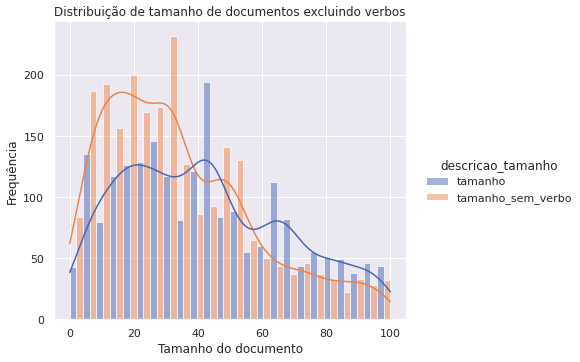
\includegraphics[scale=0.75]{explore/resources/wp_comparacao_distribuicao_tamanhos_kde_max100.png}

\vspace{3mm} %3mm

Para referência segue a distribuição sem limitar o tamanho máximo de tokens no eixo x.

\vspace{3mm} %3mm

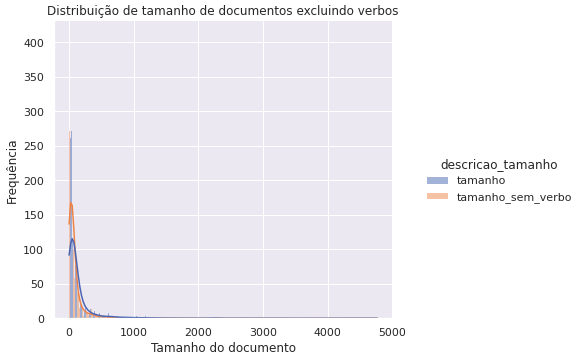
\includegraphics[scale=0.75]{explore/resources/wp_comparacao_distribuicao_tamanhos_kde.png}

\vspace{3mm} %3mm

Em seguida fiz um levantamento dos 20 tokens mais frequentes ao longo de todo o dicionário. Sem remoção de verbo a lista é:

\begin{lstlisting}
    [('est', 3996), ('reg', 3551), ('áre', 3237), ('local', 2966), ('parqu', 2893), ('rio', 2765), ('brasil', 2543), ('part', 2367), ('grand', 2043), ('cidad', 1811), ('nacion', 1765), ('sul', 1762), ('popul', 1708), ('ilh', 1630), ('mai', 1605), ('nort', 1587), ('ano', 1565), ('argentin', 1507), ('outr', 1480), ('form', 1473)]
\end{lstlisting}

Após a remoção dos verbos em língua portuguesa os 20 mais frequentes foram:

\begin{lstlisting}
    [('áre', 3237), ('parqu', 2893), ('rio', 2765), ('brasil', 2543), ('grand', 2043), ('cidad', 1811), ('nacion', 1765), ('sul', 1762), ('popul', 1708), ('ano', 1565), ('argentin', 1507), ('outr', 1480), ('km2', 1467), ('águ', 1449), ('espéci', 1271), ('provínc', 1214), ('americ', 1144), ('tod', 1087), ('municípi', 1075), ('unid', 1039)]    
\end{lstlisting}

E por mas não menos importante fiz a análise estatística do tamanho dos documentos do conjunto de páginas e percebi que a quantidade de documentos
considerados pequenos para LDA é grande. Como esta base é usada apenas para comparação e não para treinamento eu mantive os documentos pequenos.

\begin{center}
    \begin{tabular}{|c|c|c|}
        \hline
        Métrica & Tamanho Original & Tamanho sem Verbo \\
        \hline
        count & 3016.000000 & 3016.000000 \\
        \hline
        mean & 155.669430 & 96.593170 \\
        \hline
        std & 441.581739 & 257.269247 \\
        \hline
        min & 0.000000 & 0.000000 \\
        \hline
        5\% & 8.000000 & 5.000000 \\
        \hline
        10\% & 15.000000 & 10.000000 \\
        \hline
        25\% & 29.000000 & 20.000000 \\
        \hline
        50\% & 58.000000 & 37.000000 \\
        \hline
        75\% & 123.000000 & 81.000000 \\
        \hline
        90\% & 306.000000 & 197.000000 \\
        \hline
        95\% & 598.000000 & 349.250000 \\
        \hline
        max & 10018.000000 & 5699.000000 \\
        \hline
    \end{tabular}
\end{center}
